\chapter{Tráfico de membranas y clasificación de proteínas}\label{ch:b3:membrane-traffic}

Una célula del páncreas fabrica unos diez millones de moléculas de enzima
digestiva por minuto, las empaqueta en gránulos y las libera a un
conducto cuando el intestino da la señal --- sin dejar suelta jamás una
sola molécula de tripsina en su propio citoplasma. Una célula hepática
retira colesterol de la sangre tragándose enteras las partículas que lo
transportan, a razón de miles por minuto, y devuelve cada receptor a la
superficie para el siguiente. Una proteína recién fabricada destinada a
la mitocondria, al núcleo, al \omterm{def:b3:membrane-traffic:endocytosis}{lisosoma}, a la membrana o al exterior llega
a su dirección entre una docena de compartimentos con una tasa de error
que avergonzaría a un servicio de correos. Este capítulo trata de esa
clasificación: las señales escritas en las proteínas, las máquinas que
las leen, las vesículas que llevan membrana y carga entre compartimentos,
las \omterm{def:b3:membrane-traffic:coats}{cubiertas} que dan forma a las vesículas y las proteínas que las hacen
fusionarse con la diana correcta, y el tráfico en dos sentidos ---
secreción hacia fuera, endocitosis hacia dentro --- que una célula
eucariota mantiene cada segundo de su vida.

\section{Señales y direcciones}

\begin{definition}[Señales de clasificación]\label{def:b3:membrane-traffic:signals}
\index{señal de clasificación}\index{péptido señal}\index{señal de localización nuclear}\index{presecuencia}
Una \emph{señal de clasificación} es un segmento de una proteína, o una
modificación suya, que lee un receptor que entrega la proteína a un
compartimento. El \emph{péptido señal}, un tramo de \numrange{15}{30}
residuos del extremo amino con un núcleo hidrófobo, envía una proteína al
retículo endoplasmático mientras se está fabricando; desde allí la ruta
por defecto lleva a través del Golgi hasta la membrana plasmática o el
exterior, y otras señales la desvían al \omterm{def:b3:membrane-traffic:endocytosis}{lisosoma} (un azúcar fosforilado)
o de vuelta al retículo (la secuencia carboxiterminal KDEL). Una
\emph{señal de localización nuclear}, un parche básico corto como PKKKRKV,
la unen importinas que llevan la proteína plegada a través del poro
nuclear; una \emph{presecuencia} mitocondrial, una hélice anfipática de
\numrange{20}{50} residuos, la reconocen receptores de la membrana
externa y se enhebra, desplegada, por las translocasas de ambas
membranas; las enzimas peroxisómicas acaban en SKL. Las proteínas sin
ninguna de estas señales se quedan en el citosol. Toda señal se encontró
del mismo modo: suprimirla deja la proteína en el citosol, e injertarla
en una proteína citosólica envía a esa proteína al compartimento.
\end{definition}

\begin{proof}[Evidencia]
Blobel y Dobberstein (1975) tradujeron el ARN mensajero de una cadena
ligera de anticuerpo en un sistema libre de células. Sin membranas el
producto era unos veinte residuos más largo que la proteína secretada;
con fragmentos de retículo endoplasmático añadidos \emph{durante} la
traducción, el producto tenía el tamaño de la secretada y estaba
protegido de la proteasa añadida --- estaba dentro de las vesículas ---,
mientras que las membranas añadidas después de la traducción no hacían
nada. El segmento aminoterminal adicional, el \omterm{def:b3:membrane-traffic:signals}{péptido señal}, hace falta
para entrar en el retículo, se retira dentro de él y solo funciona
mientras se fabrica la cadena: la \emph{hipótesis de la señal},
confirmada en todos sus detalles cuando se purificaron el receptor (la
partícula de reconocimiento de la señal, Walter y Blobel, 1981) y el
canal (Sec61).
\end{proof}

\begin{omfigure}
\begin{tikzpicture}[every node/.style={font=\scriptsize}, >=stealth]
  % ER membrane
  \fill[omDef!15] (0,0) rectangle (12,-1.6);
  \draw[very thick, omDef] (0,0) -- (12,0); \draw[very thick, omDef] (0,-0.35) -- (12,-0.35);
  \node[right, omDef!70!black] at (0.1,-1.3) {luz del RE};
  \node[right] at (0.1,2.9) {citosol};
  % stage 1: ribosome with emerging signal peptide + SRP
  \draw[thick, fill=gray!25] (1.4,1.6) circle (0.5); \draw[thick, fill=gray!25] (1.4,0.95) ellipse (0.62 and 0.3);
  \draw[very thick, omThm] (1.4,0.65) -- (1.4,0.2) -- (1.9,0.1);
  \draw[thick, fill=omProp!40] (2.1,0.35) ellipse (0.35 and 0.2); \node[above right] at (2.2,0.5) {SRP};
  \node[below, align=center] at (1.7,-1.7) {1. asoma el péptido señal;\\la SRP se une, la traducción se pausa};
  % stage 2: docking at SRP receptor and translocon
  \draw[->, thick] (3.2,1.2) -- (4.2,1.2);
  \draw[thick, fill=gray!25] (5.6,1.75) circle (0.5); \draw[thick, fill=gray!25] (5.6,1.1) ellipse (0.62 and 0.3);
  \draw[thick, fill=omMeth!40] (5.2,0.0) rectangle (5.45,-0.35); \draw[thick, fill=omMeth!40] (5.75,0.0) rectangle (6.0,-0.35);
  \node[below, align=center] at (5.9,-1.7) {2. el receptor de SRP lo acopla\\a Sec61; la SRP se marcha};
  \draw[very thick, omThm] (5.6,0.8) -- (5.6,-0.2);
  \draw[thick, fill=omProp!40] (4.7,0.15) ellipse (0.3 and 0.18); \node[above] at (4.7,0.33) {receptor de SRP};
  % stage 3: translocation, cleavage, glycosylation
  \draw[->, thick] (7.2,1.2) -- (8.2,1.2);
  \draw[thick, fill=gray!25] (9.6,1.75) circle (0.5); \draw[thick, fill=gray!25] (9.6,1.1) ellipse (0.62 and 0.3);
  \draw[thick, fill=omMeth!40] (9.2,0.0) rectangle (9.45,-0.35); \draw[thick, fill=omMeth!40] (9.75,0.0) rectangle (10.0,-0.35);
  \draw[very thick, omThm] (9.6,0.8) -- (9.6,-0.5) .. controls (9.6,-1.0) and (10.3,-1.1) .. (10.6,-0.7);
  \draw[omThm, thick] (10.9,-0.9) -- (11.2,-0.9); \node[right, font=\tiny] at (11.0,-1.15) {señal cortada};
  \fill[omExo] (10.3,-1.0) circle (0.07); \fill[omExo] (10.45,-1.12) circle (0.07); \node[below, font=\tiny] at (10.2,-1.15) {azúcares};
  \node[below, align=center] at (10.0,-1.7) {3. la cadena cruza mientras se fabrica;\\señal cortada, azúcares añadidos};
\end{tikzpicture}

{\small La hipótesis de la señal. La partícula de reconocimiento de la
señal une el \omterm{def:b3:membrane-traffic:signals}{péptido señal} situado al principio de la cadena naciente,
pausa la traducción y acopla el ribosoma al canal Sec61; la cadena cruza
entonces la membrana a medida que se sintetiza, la señal se corta en la
luz y se añaden azúcares.}
\end{omfigure}

\begin{proposition}[Proteínas de membrana y topología]\label{prop:b3:membrane-traffic:topology}
\index{secuencia de parada de transferencia}\index{topología de membrana}
Un tramo hidrófobo de unos veinte residuos situado en medio de una cadena
que se está translocando actúa como \emph{\omterm{prop:b3:membrane-traffic:topology}{secuencia de parada de
transferencia}}: el canal se abre lateralmente y lo suelta en la bicapa
como hélice transmembranaria, con la parte ya translocada en la luz y el
resto fabricado hacia el citosol. Un segundo tramo de este tipo reanuda
la translocación, y una proteína con $n$ señales alternantes acaba con
$n$ hélices que atraviesan la membrana. La orientación fijada en el
retículo no cambia nunca: lo que da a la luz del retículo da a la luz del
Golgi y de toda vesícula posterior, y al \emph{exterior} de la célula
tras la fusión con la membrana plasmática. De ahí que los azúcares,
añadidos solo en la luz, estén siempre en la cara extracelular de una
proteína de superficie, y que la topología de un receptor pueda leerse a
partir de dónde caen sus sitios de glicosilación.
\end{proposition}

\begin{method}[Pulso y caza]\label{met:b3:membrane-traffic:pulse-chase}
\index{pulso y caza}\index{autorradiografía}
Para seguir una población de moléculas recién fabricadas por la célula:
(1) expóngase brevemente a las células (el \emph{pulso}, de unos pocos
minutos) a un precursor radiactivo o marcado de otro modo --- leucina
tritiada para las proteínas; (2) sustitúyase por un exceso de precursor
sin marcar (la \emph{caza}), de modo que no se incorpore marca nueva;
(3) fíjense muestras de células a intervalos y localícese la marca por
autorradiografía en micrografías electrónicas, o aislando los
compartimentos y contando; (4) represéntese la fracción de marca de cada
compartimento frente al tiempo. El orden en que los compartimentos se
llenan y se vacían es la ruta; los tiempos dan la permanencia en cada
uno. El laboratorio de Palade (años sesenta) lo aplicó a la célula acinar
pancreática y encontró la marca en el retículo rugoso a los \qty{3}{min},
en el Golgi a los \qty{20}{min}, en vacuolas de condensación y gránulos a
los \qty{40}{min} y en el conducto al cabo de una hora y de una señal: la
vía secretora, desplegada en el tiempo.
\end{method}

\begin{theorem}[Compartimentos sucesivos y las curvas de pulso y caza]\label{thm:b3:membrane-traffic:pulse-chase}
\index{modelo de compartimentos}
Supóngase que un pulso de proteína marcada sale del compartimento $A$
hacia $B$ con velocidad de primer orden $k_{1}$ y sale de $B$ hacia $C$
con velocidad $k_{2}$, y que $C$ la retiene. Con toda la marca en $A$ en
$t = 0$,
\[
A(t) = e^{-k_{1}t},\qquad
B(t) = \frac{k_{1}}{k_{2} - k_{1}}\bigl(e^{-k_{1}t} - e^{-k_{2}t}\bigr),
\qquad
C(t) = 1 - A - B,
\]
y la marca de $B$ alcanza su máximo en
$t^{*} = \ln(k_{2}/k_{1})/(k_{2} - k_{1})$. El tiempo medio de
permanencia en $A$ es $1/k_{1}$ y en $B$ es $1/k_{2}$, sea cual sea el
orden de las dos velocidades.
\end{theorem}
\begin{proof}
$\mathrm{d}A/\mathrm{d}t = -k_{1}A$ da la exponencial. Para $B$,
$\mathrm{d}B/\mathrm{d}t = k_{1}A - k_{2}B = k_{1}e^{-k_{1}t} - k_{2}B$;
pruébese $B = \beta(e^{-k_{1}t} - e^{-k_{2}t})$: la derivada es
$\beta(-k_{1}e^{-k_{1}t} + k_{2}e^{-k_{2}t})$ y $-k_{2}B = \beta(-k_{2}
e^{-k_{1}t} + k_{2}e^{-k_{2}t})$, de modo que la ecuación exige $\beta(k_{2}
- k_{1})e^{-k_{1}t} = k_{1}e^{-k_{1}t}$, $\beta = k_{1}/(k_{2} -
k_{1})$, y $B(0) = 0$ como se pedía. Igualando
$\mathrm{d}B/\mathrm{d}t =
0$: $k_{1}e^{-k_{1}t} = k_{2}e^{-k_{2}t}$, de donde $t^{*}$. El tiempo
medio que una molécula pasa en un compartimento del que sale a velocidad
$k$ es $\int_{0}^{
\infty} t\,k e^{-kt}\,\mathrm{d}t = 1/k$.
\end{proof}

\begin{example}[La célula de Palade en números]\label{ex:b3:membrane-traffic:palade}
Tómense $k_{1} = \qty{0.1}{min^{-1}}$ (diez minutos en el retículo) y
$k_{2} = \qty{0.05}{min^{-1}}$ (veinte en el Golgi). El Golgi alcanza su
máximo en $t^{*} = \ln 2/0.05 = \qty{13.9}{min}$, y contiene entonces
$B = 2(e^{-1.39} -
e^{-0.69}) = 2(0.25 - 0.50)\cdot(-1) = 0.50$: la mitad de la marca. A los
\qty{40}{min}, $A = 0.018$, $B = 2(0.018 - 0.135) \to 0.23$ y $C = 0.75$:
tres cuartas partes de la proteína han llegado a los gránulos. Las curvas
observadas en el laboratorio de Palade tienen esta forma, y ajustarlas
fue como se midieron por primera vez los tiempos de permanencia.
\end{example}

\begin{omfigure}
\begin{tikzpicture}
\begin{axis}[
  width=0.7\linewidth, height=5.6cm,
  axis x line=bottom, axis y line=left,
  xmin=0, xmax=80, ymin=0, ymax=1.05,
  xlabel={minutos tras el pulso}, ylabel={fracción de la marca},
  xlabel style={font=\small, at={(axis description cs:0.5,-0.12)}, anchor=north},
  ylabel style={font=\small},
  tick label style={font=\small}, xtick={0,20,40,60,80}, ytick={0,0.5,1},
  clip=false,
]
\addplot[very thick, omDef, domain=0:80, samples=80] {exp(-0.1*x)};
\addplot[very thick, omProp, domain=0:80, samples=80] {2*(exp(-0.05*x)-exp(-0.1*x))};
\addplot[very thick, omMeth!70!black, domain=0:80, samples=80] {1-exp(-0.1*x)-2*(exp(-0.05*x)-exp(-0.1*x))};
\node[font=\scriptsize, omDef, anchor=south west] at (axis cs:4,0.62) {retículo, $A$};
\node[font=\scriptsize, omProp, anchor=south] at (axis cs:14,0.53) {Golgi, $B$};
\node[font=\scriptsize, omMeth!70!black, anchor=north west] at (axis cs:45,0.72) {gránulos, $C$};
\end{axis}
\end{tikzpicture}

{\small Curvas de \omterm{met:b3:membrane-traffic:pulse-chase}{pulso y caza} del modelo de dos velocidades con $k_{1} =
\qty{0.1}{min^{-1}}$ y $k_{2} = \qty{0.05}{min^{-1}}$: la marca sale del
retículo exponencialmente, pasa por el Golgi con un máximo a los
\qty{14}{min} y se acumula en los gránulos.}
\end{omfigure}

\section{El retículo endoplasmático: plegamiento, azúcares y calidad}

\begin{definition}[N-glicosilación y control de calidad]\label{def:b3:membrane-traffic:glycosylation}
\index{N-glicosilación}\index{ciclo de la calnexina}\index{degradación asociada al RE}\index{respuesta a proteínas desplegadas}
Al entrar la cadena en la luz se transfiere desde un transportador
lipídico a las asparaginas de la secuencia Asn-X-Ser/Thr un
oligosacárido preensamblado de catorce azúcares (dos
N-acetilglucosaminas, nueve manosas, tres glucosas): la
\emph{N-glicosilación}. Las tres glucosas se recortan luego una a una, y
ese recorte es un reloj del plegamiento: una proteína que aún lleva una
glucosa la retiene la \omterm{def:b3:structural-biology:chaperones}{chaperona} calnexina; una proteína a la que se ha
quitado la última glucosa pero que todavía no está plegada la vuelve a
glucosilar una enzima que reconoce parches hidrófobos expuestos, y
regresa a la calnexina --- el \emph{ciclo de la calnexina}. Las proteínas
que fracasan una y otra vez se devuelven al citosol, se ubiquitinan y las
destruye el proteasoma: la \emph{degradación asociada al RE} (ERAD).
Cuando las proteínas desplegadas se acumulan más deprisa de lo que pueden
plegarse o destruirse, unos sensores de la membrana del retículo lanzan
la \emph{respuesta a proteínas desplegadas}: se frena la traducción, se
inducen los genes de \omterm{def:b3:structural-biology:chaperones}{chaperonas}, se expande el retículo y, si el estrés
persiste, se mata la célula. La mutación más frecuente de la fibrosis
quística ($\Delta$F508 en CFTR) produce un canal que funcionaría pero que
se pliega demasiado despacio, lo atrapa la ERAD y nunca llega a la
superficie; los fármacos que le ayudan a plegarse son hoy un tratamiento.
\end{definition}

\begin{omfigure}
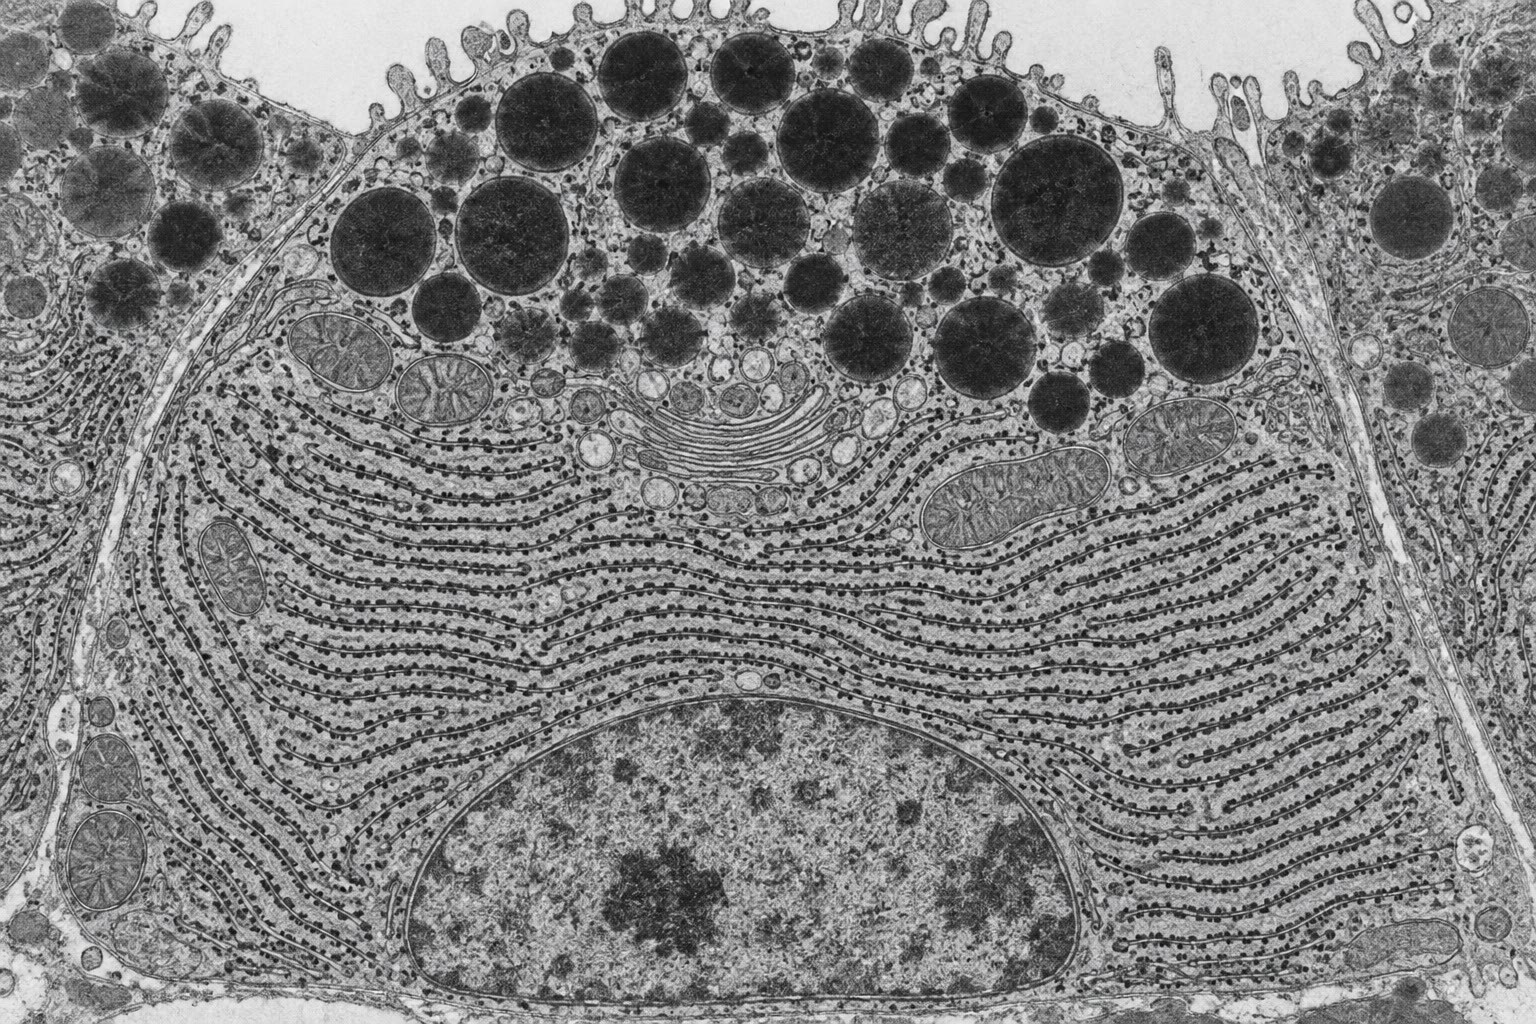
\includegraphics[width=0.56\linewidth]{images/book5/ai/b5-08-pancreas-acinar.jpg}

{\small Una célula acinar pancreática al microscopio electrónico: el
retículo endoplasmático rugoso apilado y tachonado de ribosomas llena la
base, el Golgi se sitúa sobre el núcleo y los densos gránulos de
secreción de enzima digestiva se apiñan bajo la superficie apical, a la
espera de una señal.}
\end{omfigure}

\section{Vesículas: gemación, direccionamiento, fusión}

\begin{definition}[Cubiertas y gemación de vesículas]\label{def:b3:membrane-traffic:coats}
\index{vesícula cubierta}\index{COPII}\index{COPI}\index{clatrina}\index{GTPasa pequeña}
Una vesícula de transporte la moldea una \emph{cubierta} de proteínas
ensamblada en la cara citosólica de una membrana, que la curva formando
una yema de \qtyrange{60}{100}{nm}, recoge la carga mediante receptores
que atraviesan la membrana y se desprende una vez que la vesícula se ha
estrangulado. Tres cubiertas sirven a las rutas principales:
\emph{COPII} para las vesículas que salen del retículo hacia el Golgi,
\emph{COPI} para el tráfico de regreso del Golgi al retículo y entre
cisternas del Golgi, y la \emph{clatrina} --- una proteína de tres patas
que polimeriza en una jaula de hexágonos y pentágonos --- para las
vesículas que salen del Golgi trans hacia los \omterm{def:b3:membrane-traffic:endocytosis}{endosomas} y para la
endocitosis en la membrana plasmática, donde unas proteínas adaptadoras
enlazan la jaula con los receptores que se internalizan. Cada cubierta la
recluta una \emph{GTPasa pequeña} (Sar1 para COPII, Arf1 para COPI y la
clatrina) que se inserta en la membrana en su forma con GTP y que, al
hidrolizar el GTP tras la gemación, deja caer la cubierta. Las señales de
recuperación mantienen distintos los compartimentos: a las proteínas del
retículo que se escapan llevando KDEL las une en el Golgi un receptor y
las devuelve en vesículas COPI.
\end{definition}

\begin{omfigure}
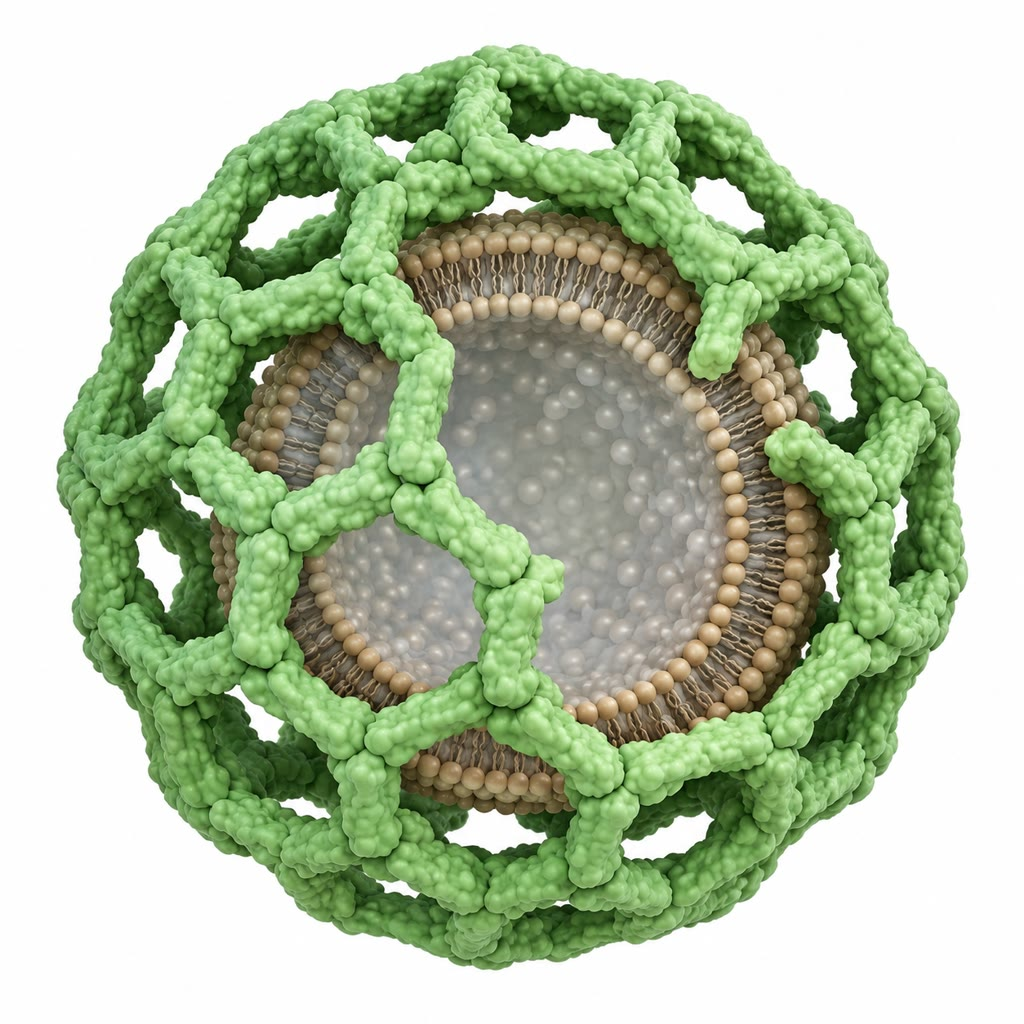
\includegraphics[width=0.36\linewidth]{images/book5/ai/b5-08-clathrin-cage.jpg}\hspace{0.04\linewidth}
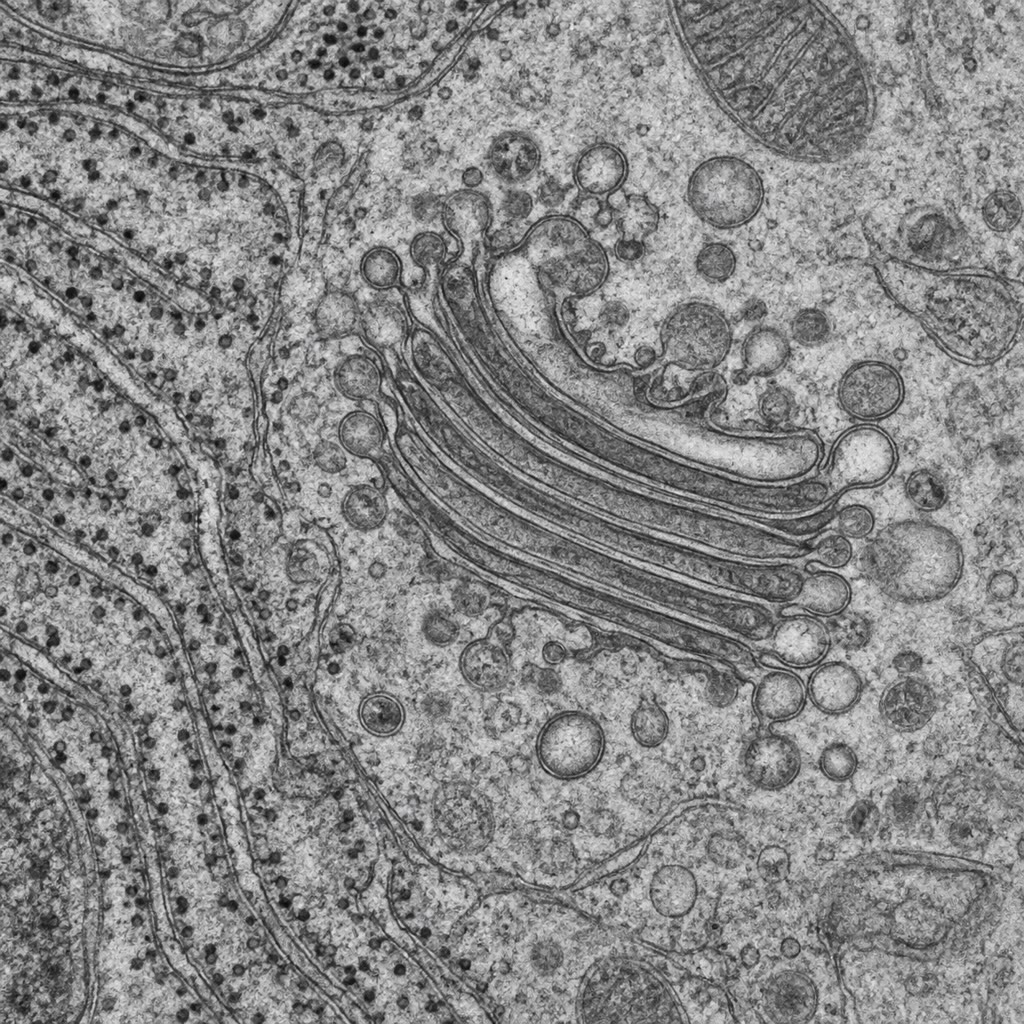
\includegraphics[width=0.36\linewidth]{images/book5/ai/b5-08-golgi-tem.jpg}

{\small Izquierda: una jaula de \omterm{def:b3:membrane-traffic:coats}{clatrina}, la red poliédrica de unidades
de tres patas que da forma a una vesícula endocítica (recortada para
mostrar la membrana del interior). Derecha: una pila de Golgi al
microscopio electrónico, un montón de cisternas aplanadas con vesículas
gemando en los bordes.}
\end{omfigure}

\begin{definition}[Direccionamiento y fusión]\label{def:b3:membrane-traffic:fusion}
\index{GTPasa Rab}\index{SNARE}\index{fusión de membranas}\index{sinaptotagmina}
Una vesícula encuentra su diana por dos capas de reconocimiento. Las
\emph{GTPasas Rab} --- unas sesenta en una célula humana, cada una en las
membranas de un compartimento --- reclutan proteínas de amarre largas que
atrapan la vesícula entrante que lleva la Rab correspondiente. Actúan
después las \emph{SNARE}: una v-SNARE de la vesícula y unas t-SNARE de la
diana, proteínas helicoidales ancladas en sus membranas, se enrollan una
en torno a otra desde sus extremos distales hacia las membranas, y la
energía del haz de cuatro hélices que forman junta las dos bicapas hasta
que se fusionan. Cada emparejamiento de SNARE es específico, una segunda
comprobación de la dirección. Tras la fusión el haz lo separa la ATPasa
NSF para reutilizarlo. La fusión puede hacerse esperar a una señal: en el
terminal nervioso las SNARE quedan enrolladas a medias por la complexina
hasta que la \emph{sinaptotagmina}, al unir el calcio que entra cuando
llega un potencial de acción, completa el enrollamiento en menos de un
milisegundo --- la liberación de neurotransmisor tratada en el volumen de
segundo año. Las neurotoxinas del tétanos y del botulismo son proteasas
que cortan SNARE.
\end{definition}

\begin{proof}[Evidencia]
Novick y Schekman (1980) aislaron mutantes de levadura sensibles a la
temperatura que dejaban de secretar a \qty{37}{\celsius} y acumulaban
proteína en el compartimento que su defecto bloqueara --- retículo, Golgi
o vesículas apiladas bajo la superficie; los $23$ genes \emph{sec}
definieron los pasos y, una vez clonados, resultaron codificar las
\omterm{def:b3:membrane-traffic:coats}{cubiertas}, las GTPasas y las \omterm{def:b3:membrane-traffic:fusion}{SNARE}. Rothman reconstituyó el transporte
entre cisternas del Golgi en un tubo de ensayo con membranas purificadas,
citosol y ATP, y de ahí purificó la NSF y las \omterm{def:b3:membrane-traffic:fusion}{SNARE}; los dos enfoques
convergieron en las mismas proteínas, y las máquinas de la levadura y del
mamífero resultaron ser la misma.
\end{proof}

\begin{omfigure}
\begin{tikzpicture}[every node/.style={font=\scriptsize}, >=stealth]
  % three stages left to right
  \foreach \x/\gap/\lab in {0/1.2/{1. amarrada por Rab}, 4.4/0.55/{2. las SNARE se enrollan}, 8.8/0.0/{3. fusión, carga liberada}} {
    % target membrane
    \draw[very thick, omDef] (\x,0) -- (\x+3.4,0); \draw[very thick, omDef] (\x,-0.3) -- (\x+3.4,-0.3);
    \node[below, align=center] at (\x+1.7,-0.45) {\lab};
  }
  % stage 1 vesicle
  \draw[very thick, omProp] (1.7,1.2+0.8) circle (0.8); \draw[very thick, omProp] (1.7,1.2+0.8) circle (0.6);
  \draw[omThm, thick] (1.4,1.25) -- (1.4,0.35); \draw[omThm, thick] (2.0,1.25) -- (2.0,0.35);
  \draw[omMeth!70!black, thick] (1.7,1.2) -- (1.7,0.6); \draw[omMeth!70!black, thick] (1.7,0.6) -- (1.7,0.0);
  \draw[thick, fill=omExo!40] (0.7,0.9) ellipse (0.25 and 0.2); \node[left] at (0.45,0.9) {Rab};
  \draw[thick, omExo!70!black] (0.95,0.9) .. controls (1.1,0.5) .. (1.2,0.05); \node[left, font=\tiny] at (0.9,0.4) {amarre};
  \node[right, font=\tiny] at (2.05,0.8) {SNARE};
  % stage 2 vesicle closer, helices twisted
  \draw[very thick, omProp] (6.1,0.55+0.8) circle (0.8); \draw[very thick, omProp] (6.1,0.55+0.8) circle (0.6);
  \draw[omThm, very thick] (5.85,0.6) .. controls (6.2,0.5) and (5.9,0.3) .. (6.1,0.05);
  \draw[omMeth!70!black, very thick] (6.35,0.6) .. controls (6.0,0.5) and (6.3,0.3) .. (6.1,0.05);
  \node[right, font=\tiny, align=left] at (6.6,0.35) {el haz de cuatro hélices\\junta las membranas};
  % stage 3 fused omega shape
  \draw[very thick, omProp] (9.7,0) .. controls (9.7,1.5) and (11.3,1.5) .. (11.3,0);
  \draw[very thick, omProp] (9.9,-0.3) .. controls (9.9,1.1) and (11.1,1.1) .. (11.1,-0.3);
  \foreach \p in {(10.5,-0.9),(10.2,-1.1),(10.8,-1.15)} \fill[omExo] \p circle (0.06);
  \draw[->, omExo, thick] (10.5,0.5) -- (10.5,-0.6);
  \node[right, font=\tiny, align=left] at (11.4,0.8) {después la NSF\\desenrolla las\\SNARE};
\end{tikzpicture}

{\small La fusión en tres pasos. Una Rab de la vesícula y un amarre de la
diana ponen las dos membranas al alcance; las \omterm{def:b3:membrane-traffic:fusion}{SNARE} de la vesícula y de
la diana (rojo y verde) se enrollan en un haz de cuatro hélices que
arrastra las bicapas una contra otra; se fusionan y la carga entra en el
compartimento de destino.}
\end{omfigure}

\begin{proposition}[El Golgi]\label{prop:b3:membrane-traffic:golgi}
\index{aparato de Golgi}\index{maduración cisternal}\index{manosa-6-fosfato}
El Golgi es una pila de cuatro a ocho cisternas aplanadas, con la cara
cis hacia el retículo y la cara trans hacia la membrana plasmática, y
cada cisterna alberga un conjunto distinto de enzimas que recortan y
reconstruyen los azúcares de las glicoproteínas que pasan y añaden
azúcares unidos por O, sulfato y fosfato. La carga avanza sobre todo por
\emph{\omterm{prop:b3:membrane-traffic:golgi}{maduración cisternal}}: una cisterna nueva se forma en la cara cis a
partir de las vesículas que llegan, recorre la pila como lo hicieron las
anteriores y madura a medida que las vesículas \omterm{def:b3:membrane-traffic:coats}{COPI} llevan hacia atrás
las enzimas de cada cisterna a la más joven que la sigue; en la cara
trans se deshace en vesículas con destino propio. Allí se decide la
clasificación: las hidrolasas lisosómicas, marcadas en el Golgi cis con
\emph{manosa-6-fosfato}, las une su receptor y se empaquetan en vesículas
de \omterm{def:b3:membrane-traffic:coats}{clatrina} hacia el \omterm{def:b3:membrane-traffic:endocytosis}{endosoma}; las proteínas de secreción regulada se
agregan al pH ligeramente ácido en gránulos de condensación; y todo lo
demás sale en la corriente constitutiva hacia la superficie. En la
enfermedad de las células~I falta la enzima que fosforila, las hidrolasas
se secretan en lugar de entregarse y los \omterm{def:b3:membrane-traffic:endocytosis}{lisosomas} se llenan de material
sin digerir.
\end{proposition}

\begin{omfigure}
\begin{tikzpicture}[every node/.style={font=\scriptsize}, >=stealth]
  % plasma membrane top
  \draw[very thick, omDef] (0,4.2) -- (12,4.2); \node[above] at (6,4.25) {membrana plasmática \quad (el exterior, arriba)};
  % ER
  \draw[thick, fill=omDef!12] (0.3,0.0) rectangle (4.0,0.9); \node at (2.15,0.45) {retículo endoplasmático};
  % Golgi stack
  \foreach \y in {1.5,1.85,2.2,2.55} \draw[thick, fill=omProp!25] (4.8,\y) ellipse (1.4 and 0.13);
  \node[right] at (6.3,1.5) {cis}; \node[left] at (3.35,2.55) {trans};
  \node[right] at (6.3,2.05) {pila de Golgi};
  % ER -> Golgi (COPII)
  \draw[->, thick, omMeth!70!black] (3.9,0.95) -- (4.5,1.4); \node[right, omMeth!70!black, font=\tiny] at (4.35,1.02) {COPII};
  % Golgi -> ER (COPI)
  \draw[->, thick, omThm] (3.6,1.42) -- (2.9,0.95); \node[left, omThm, font=\tiny] at (2.95,1.3) {COPI, recuperación KDEL};
  % trans Golgi -> PM constitutive
  \draw[->, thick, omMeth!70!black] (5.6,2.7) -- (7.6,4.1); \node[left, font=\tiny, align=right] at (6.4,3.6) {secreción\\constitutiva};
  % trans -> secretory granule -> PM regulated
  \draw[->, thick, omMeth!70!black] (4.6,2.7) -- (4.0,3.3); \draw[thick, fill=omExo!50] (3.8,3.5) circle (0.22); \draw[->, thick, omMeth!70!black] (3.8,3.75) -- (3.8,4.1);
  \node[left, font=\tiny, align=right] at (3.55,3.5) {gránulo de secreción:\\regulado, ante una señal};
  % trans -> endosome/lysosome (clathrin, M6P)
  \draw[->, thick, omProp!80!black] (6.0,2.62) -- (8.25,2.62); \node[above, font=\tiny] at (7.1,2.67) {clatrina, receptor de M6P};
  \draw[thick, fill=omProp!20] (8.8,2.7) circle (0.5); \node at (8.8,2.7) {\tiny endosoma};
  \draw[->, thick, omProp!80!black] (9.25,2.4) -- (10.2,1.95); \draw[thick, fill=omThm!25] (10.7,1.6) circle (0.5); \node at (10.7,1.6) {\tiny lisosoma};
  % endocytosis from PM to endosome
  \draw[->, thick, omDef] (9.6,4.15) -- (9.1,3.2); \node[right, font=\tiny, align=left] at (9.5,3.7) {endocitosis\\(fositas de clatrina)};
  % recycling endosome -> PM
  \draw[->, thick, omDef] (8.5,3.2) -- (8.0,4.15); \node[left, font=\tiny] at (8.3,3.3) {reciclado};
  % lysosome inputs autophagy
  \draw[->, thick, gray] (11.9,0.6) -- (11.1,1.3); \node[below, font=\tiny, align=center] at (11.9,0.55) {autofagosoma\\(citoplasma, orgánulos)};
\end{tikzpicture}

{\small El mapa del tráfico de membranas. Hacia fuera (verde): del
retículo al Golgi en vesículas \omterm{def:b3:membrane-traffic:coats}{COPII}, y del Golgi a la superficie de
forma constitutiva o a través de gránulos que esperan una señal. Hacia
atrás (rojo): las vesículas \omterm{def:b3:membrane-traffic:coats}{COPI} devuelven las proteínas del retículo que
se escaparon. Hacia abajo (naranja): las enzimas lisosómicas marcadas con
manosa-6-fosfato van al \omterm{def:b3:membrane-traffic:endocytosis}{endosoma} y al \omterm{def:b3:membrane-traffic:endocytosis}{lisosoma}. Hacia dentro (azul):
endocitosis desde la superficie, con la mayoría de los receptores
reciclados.}
\end{omfigure}

\section{Endocitosis y lisosoma}

\begin{definition}[Endocitosis]\label{def:b3:membrane-traffic:endocytosis}
\index{endocitosis mediada por receptor}\index{endosoma}\index{lisosoma}\index{autofagia}
La \emph{endocitosis mediada por receptor} concentra un ligando unido a
receptores de superficie en fositas recubiertas de \omterm{def:b3:membrane-traffic:coats}{clatrina}, que se
estrangulan (la GTPasa dinamina constriñe el cuello) como vesículas de
unos \qty{100}{nm} --- mil por minuto en un fibroblasto, lo que renueva
toda la membrana de superficie en una hora. Las vesículas se fusionan en
\emph{endosomas tempranos}, cuya luz acidifica hasta pH~6 una bomba de
protones; la mayoría de los ligandos sueltan allí sus receptores, los
receptores vuelven a la superficie en vesículas de reciclado y el ligando
sigue viaje mientras el endosoma madura hasta endosoma tardío (pH~5.5) y
se fusiona con un \emph{lisosoma}: un compartimento a pH~4.5--5 que
contiene unas sesenta hidrolasas --- proteasas, nucleasas, lipasas,
glicosidasas --- activas solo a ese pH, de modo que una fuga al citosol
neutro hace poco daño. El lisosoma digiere además el propio material de
la célula que le entrega la \emph{autofagia}: una membrana doble crece
alrededor de una porción de citoplasma o de un orgánulo gastado, se
cierra en un autofagosoma y se fusiona con el lisosoma; los productos se
devuelven al citosol. La autofagia la induce el ayuno (recicla la propia
sustancia de la célula para obtener energía) y limpia agregados y
mitocondrias dañadas; su fallo se ha implicado en la neurodegeneración.
\end{definition}

\begin{proof}[Evidencia]
Brown y Goldstein (años setenta) siguieron la lipoproteína de baja
densidad (LDL), la partícula que transporta el colesterol en la sangre,
hasta el interior de fibroblastos en cultivo. La LDL se unía de forma
saturable a unos \num{20000} sitios de superficie por célula, se
internalizaba en minutos en fositas recubiertas, y su colesterol se
liberaba en los \omterm{def:b3:membrane-traffic:endocytosis}{lisosomas} y apagaba la síntesis de colesterol de la
propia célula. Los fibroblastos de pacientes con hipercolesterolemia
familiar no unían LDL (receptor ausente) o la unían pero no la
internalizaban (una mutación de la cola citosólica del receptor que
impide que la capturen los adaptadores de \omterm{def:b3:membrane-traffic:coats}{clatrina}): la enfermedad era un
defecto de la endocitosis, la cola del receptor contenía la señal de
internalización, y el receptor reciclado --- cada uno con centenares de
viajes de ida y vuelta --- quedó establecido como el mecanismo general de
captación.
\end{proof}

\begin{proposition}[Captación mediante receptores reciclados]\label{prop:b3:membrane-traffic:uptake}
\index{reciclado de receptores}
Supóngase que una célula tiene $R$ receptores en total, de los cuales $S$
están en la superficie y $R - S$ dentro, de regreso. Un receptor de
superficie está ocupado con probabilidad $\theta = [L]/(K_{d} + [L])$, un
receptor ocupado se internaliza a velocidad $k_{i}$, y un receptor
internalizado regresa a velocidad $k_{r}$. En el estado estacionario el
flujo de ligando hacia la célula es
\[
J = \frac{R\,k_{i}k_{r}\,\theta}{k_{r} + k_{i}\theta},
\]
que satura, a medida que sube la concentración de ligando, en $J_{\max} =
R\,k_{i}k_{r}/(k_{i} + k_{r})$: la captación de una célula no la limitan
sus receptores por sí solos, sino la rapidez con que puede traerlos de
vuelta.
\end{proposition}
\begin{proof}
Los receptores de superficie se pierden a velocidad $k_{i}\theta S$ y se
recuperan a velocidad $k_{r}(R - S)$; en el estado estacionario ambas se
compensan, luego $S = R\,k_{r}/(k_{r}
+ k_{i}\theta)$. Cada internalización lleva un ligando, de modo que $J =
k_{i}\theta S$, lo que da la fórmula. Cuando $\theta \to 1$ el flujo
tiende a $R\,k_{i}k_{r}/(k_{r} + k_{i})$ --- los receptores ciclan tan
deprisa como permiten las dos velocidades, con una fracción
$k_{r}/(k_{i} + k_{r})$ de ellos en la superficie en cada instante.
\end{proof}

\begin{example}[Colesterol partícula a partícula]\label{ex:b3:membrane-traffic:ldl}
Un fibroblasto con $R = \num{20000}$ receptores de LDL, un tiempo de
internalización de \qty{5}{min} ($k_{i} = \qty{0.2}{min^{-1}}$) y un
tiempo de regreso de \qty{10}{min}
($k_{r} = \qty{0.1}{min^{-1}}$) capta, con LDL saturante,
$J_{\max} = \num{20000}\times 0.2\times 0.1/0.3 \approx 1300$ partículas
por minuto, con un tercio de sus receptores en la superficie en cada
instante; cada partícula trae unas \num{1500} moléculas de colesterol,
dos millones por minuto, suficientes para construir alrededor de una
décima de micrómetro cuadrado de membrana. Un heterocigoto para la
hipercolesterolemia familiar, con la mitad de los receptores, capta la
mitad; el colesterol en sangre se duplica y la cardiopatía llega veinte
años antes. Las estatinas suben $R$ al privar a la célula hepática de su
propio colesterol.
\end{example}

\begin{omfigure}
\begin{tikzpicture}
\begin{axis}[
  width=0.7\linewidth, height=5.4cm,
  axis x line=bottom, axis y line=left,
  xmin=0, xmax=10, ymin=0, ymax=1500,
  xlabel={concentración de LDL, $[L]/K_{d}$}, ylabel={partículas por minuto},
  xlabel style={font=\small, at={(axis description cs:0.5,-0.12)}, anchor=north},
  ylabel style={font=\small},
  tick label style={font=\small}, xtick={0,2,4,6,8,10}, ytick={0,500,1000,1333}, yticklabels={0,500,1000,$J_{\max}$},
  clip=false,
]
\addplot[very thick, omDef, domain=0:10, samples=60] {20000*0.2*0.1*(x/(1+x))/(0.1+0.2*(x/(1+x)))};
\addplot[very thick, omThm, domain=0:10, samples=60] {10000*0.2*0.1*(x/(1+x))/(0.1+0.2*(x/(1+x)))};
\addplot[dashed, gray, domain=0:10, samples=2] {1333};
\node[font=\scriptsize, omDef, anchor=north west] at (axis cs:4,900) {$R = \num{20000}$};
\node[font=\scriptsize, omThm, anchor=north west] at (axis cs:4,560) {$R = \num{10000}$ (heterocigoto)};
\end{axis}
\end{tikzpicture}

{\small Captación de LDL mediante receptores reciclados, con la fórmula
de la proposición y $k_{i} = \qty{0.2}{min^{-1}}$ y $k_{r} =
\qty{0.1}{min^{-1}}$: satura con el ligando, y se reduce a la mitad
cuando falta la mitad de los receptores.}
\end{omfigure}

\begin{remark}[Una membrana, muchos compartimentos]\label{rem:b3:membrane-traffic:one-membrane}
Toda membrana del sistema secretor y endocítico es, topológicamente, una
sola membrana: la luz del retículo es continua, a través de vesículas,
con el exterior de la célula, y un lípido o una proteína fabricados en el
retículo pueden llegar a la superficie sin cruzar nunca una bicapa. Lo
que mantiene distintos los compartimentos no son paredes sino tráfico ---
empaquetado selectivo hacia fuera, recuperación selectiva hacia atrás y
un par específico de moléculas de reconocimiento en cada fusión. Los
compartimentos son estados estacionarios de flujos, como las pozas de un
río, y una célula que deja de traficar pierde su geografía en cuestión de
horas.
\end{remark}

\section{Ejercicios}

\begin{exercise}[$\star$]\label{exo:b3:membrane-traffic:1}
Dense la señal y el destino de cada una: un tramo de veinte residuos
hidrófobos en el extremo amino; PKKKRKV; una hélice anfipática
aminoterminal; KDEL en el extremo carboxilo; una manosa-6-fosfato en los
azúcares.
\end{exercise}

\begin{exercise}[$\star$]\label{exo:b3:membrane-traffic:2}
Descríbanse las tres observaciones clave del experimento de
Blobel y Dobberstein y qué mostró cada una.
\end{exercise}

\begin{exercise}[$\star$]\label{exo:b3:membrane-traffic:3}
Nómbrense la \omterm{def:b3:membrane-traffic:coats}{cubierta} y el sentido del transporte para: del retículo al
Golgi; del Golgi al retículo; del Golgi trans al \omterm{def:b3:membrane-traffic:endocytosis}{endosoma}; de la membrana
plasmática al \omterm{def:b3:membrane-traffic:endocytosis}{endosoma}.
\end{exercise}

\begin{exercise}[$\star$]\label{exo:b3:membrane-traffic:4}
¿Por qué los azúcares de una proteína de la membrana plasmática están
siempre en el exterior de la célula?
\end{exercise}

\begin{exercise}[$\star\star$]\label{exo:b3:membrane-traffic:5}
En el modelo del \cref{thm:b3:membrane-traffic:pulse-chase} con $k_{1}
= \qty{0.2}{min^{-1}}$ y $k_{2} = \qty{0.05}{min^{-1}}$, hállese cuándo
alcanza su máximo la marca del Golgi y cuánta hay en el máximo; después,
la fracción en los gránulos a los \qty{60}{min}.
\end{exercise}

\begin{exercise}[$\star\star$]\label{exo:b3:membrane-traffic:6}
Una proteína de membrana tiene tramos hidrófobos de $22$ residuos en las
posiciones 30, 90, 150 y 210 y un \omterm{def:b3:membrane-traffic:signals}{péptido señal} aminoterminal. Dibújese o
descríbase su topología: cuántas hélices, y a qué lado da cada segmento
entre ellas. ¿Dónde puede glicosilarse?
\end{exercise}

\begin{exercise}[$\star\star$]\label{exo:b3:membrane-traffic:7}
Con la \cref{prop:b3:membrane-traffic:uptake} y $R = \num{30000}$,
$k_{i} = \qty{0.25}{min^{-1}}$, $k_{r} = \qty{0.05}{min^{-1}}$,
calcúlense $J_{\max}$ y la fracción de receptores en la superficie en
saturación. ¿Qué único cambio duplicaría la captación?
\end{exercise}

\begin{exercise}[$\star\star$]\label{exo:b3:membrane-traffic:8}
Predíganse el destino de las hidrolasas lisosómicas, y el fenotipo, en
(a) una célula sin receptor de manosa-6-fosfato, (b) una célula sin la
fosfotransferasa que añade la marca, (c) una célula tratada con un
fármaco que neutraliza el pH endosómico.
\end{exercise}

\begin{exercise}[$\star\star$]\label{exo:b3:membrane-traffic:9}
La mutación JD del receptor de LDL cambia una tirosina de la cola
citosólica. Las células unen la LDL con normalidad pero no la captan.
Explíquese el mecanismo y predígase dónde se encuentran los receptores en
la superficie celular respecto a las fositas recubiertas.
\end{exercise}

\begin{exercise}[$\star\star\star$]\label{exo:b3:membrane-traffic:10}
Resuélvase el modelo de \omterm{met:b3:membrane-traffic:pulse-chase}{pulso y caza} para el caso $k_{1} = k_{2} = k$ (la
fórmula del teorema es singular ahí): muéstrese que
$B(t) = kt\,e^{-kt}$ y hállese el máximo. Explíquese después por qué
medir solo la fracción de los gránulos $C(t)$ no puede determinar las dos
velocidades por separado.
\end{exercise}

\begin{exercise}[$\star\star\star$]\label{exo:b3:membrane-traffic:11}
Un fibroblasto internaliza \num{1000} vesículas de \omterm{def:b3:membrane-traffic:coats}{clatrina} de
\qty{100}{nm} de diámetro por minuto y tiene una superficie de
\qty{3000}{\micro m^2}. ¿Cuánto tarda en internalizar el equivalente de
toda la superficie? ¿Por qué no se encoge la célula, y qué implica el
balance sobre la velocidad de exocitosis y sobre el volumen de líquido
captado por hora?
\end{exercise}

\begin{exercise}[$\star\star\star$]\label{exo:b3:membrane-traffic:12}
La toxina botulínica corta una \omterm{def:b3:membrane-traffic:fusion}{SNARE} en los terminales nerviosos
motores; la toxina tetánica corta la misma \omterm{def:b3:membrane-traffic:fusion}{SNARE} en las interneuronas
inhibidoras de la médula espinal. Explíquese por qué la primera causa una
parálisis flácida y la segunda una espástica, y por qué una toxina que
bloquea la fusión resulta útil en medicina a dosis minúsculas.
\end{exercise}

\section{Problema: un día de una célula pancreática}

\begin{problem}[{Problema de fin de semana --- el rendimiento de una
célula secretora contado en moléculas, vesículas y micrómetros cuadrados,
sus curvas de pulso y caza resueltas, la captación de colesterol de una
célula hepática calculada con receptores reciclados y un lisosoma
acidificado protón a protón, hasta llegar al momento del máximo del
Golgi, a las vesículas que geman por minuto y a las partículas de LDL
captadas por hora}]
\label{pb:b3:membrane-traffic:1}
Datos: una célula acinar fabrica $10^{7}$ moléculas de enzima por minuto,
de \qty{25}{kDa} cada una y \qty{4}{nm} de diámetro. Las vesículas de
transporte son esferas de \qty{70}{nm} de diámetro; un gránulo es una
esfera de \qty{1}{\micro m}. Área de membrana por molécula de lípido,
\qty{0.7}{nm^2}, con dos monocapas. El retículo de la célula tiene un
área de \qty{6000}{\micro m^2}. \omterm{met:b3:membrane-traffic:pulse-chase}{Pulso y caza}:
$k_{1} = \qty{0.1}{min^{-1}}$, $k_{2} = \qty{0.05}{min^{-1}}$. Una célula
hepática: $R = \num{50000}$ receptores de LDL,
$k_{i} = \qty{0.2}{min^{-1}}$, $k_{r} = \qty{0.1}{min^{-1}}$,
$K_{d} = \qty{2}{nmol/L}$, concentración plasmática de partículas de LDL
\qty{2}{nmol/L}; \num{1500} moléculas de colesterol por partícula.
Un \omterm{def:b3:membrane-traffic:endocytosis}{lisosoma}: esfera de \qty{0.5}{\micro m}, pH de $7.2$ a $4.7$, con una
capacidad tampón tal que hay que bombear $50$ protones por cada uno que
queda libre; una bomba de protones mueve $200$ protones por segundo.

\medskip
\noindent\textbf{Parte I --- Rendimiento.}
\begin{enumerate}
  \item ¿Qué masa de enzima fabrica la célula por minuto, y por día?
        Compárese con el propio contenido proteico de la célula, unos
        \qty{300}{pg}.
  \item ¿Cuántas moléculas de enzima caben en una vesícula si llenan el
        \qty{30}{\%} de su volumen (esfera de \qty{4}{nm})? ¿Cuántas
        vesículas por minuto salen del retículo?
  \item ¿Cuánta área de membrana llevan esas vesículas por minuto, y en
        cuánto tiempo consumirían todo el retículo si no volviera nada?
  \item ¿Cuántas moléculas de lípido son eso por minuto? ¿Qué ha de
        hacer la célula para conservar su retículo?
  \item ¿Cuántas moléculas de enzima caben en un gránulo con el mismo
        empaquetamiento, y cuántos gránulos llena la célula por hora?
  \item Una comida vacía $300$ gránulos en diez minutos por fusión con
        la membrana apical y añade su membrana a una superficie de
        \qty{50}{\micro m^2}. ¿Por qué factor crece la superficie
        apical, y qué ha de venir después?
\end{enumerate}

\medskip
\noindent\textbf{Parte II --- Tiempos.}
\begin{enumerate}[resume]
  \item Con las velocidades dadas, ¿cuándo alcanza su máximo la marca
        del Golgi, y qué fracción hay?
  \item ¿Qué fracción de un pulso está en el retículo, en el Golgi y en
        los gránulos a los \qty{30}{min}?
  \item ¿Tiempos medios de permanencia en los dos compartimentos? ¿Cuál
        es el tiempo total medio desde la síntesis hasta el gránulo?
  \item Un fármaco frena la salida del Golgi a
        $k_{2} = \qty{0.01}{min^{-1}}$. ¿Nuevo momento y nueva fracción
        del máximo? ¿Qué aspecto tiene el Golgi al microscopio?
  \item Explíquese por qué la fracción máxima del Golgi es
        $k_{1}/k_{2}$ elevado a una potencia (dese la potencia) y por
        tanto siempre menor que $1$.
  \item Si el paso del retículo fuera mucho más rápido que el del
        Golgi, ¿a qué tendería $B(t)$? Interprétese.
\end{enumerate}

\medskip
\noindent\textbf{Parte III --- Colesterol.}
\begin{enumerate}[resume]
  \item Calcúlense $\theta$ a la concentración plasmática de LDL y la
        captación $J$ en partículas por minuto y por hora.
  \item ¿Cuántas moléculas de colesterol por hora? Las membranas de la
        célula contienen $5\times 10^{9}$ moléculas de colesterol;
        ¿cuánto se tardaría en reemplazarlas todas solo a partir de la
        LDL?
  \item Calcúlense la fracción de receptores en la superficie y el
        número de viajes de ida y vuelta que hace cada receptor en sus
        \qty{20}{h} de vida.
  \item Un heterocigoto tiene $R = \num{25000}$: recalcúlese $J$. La LDL
        plasmática sube hasta que la captación iguala a la producción:
        ¿por qué factor, si $\theta$ está muy por debajo de la
        saturación?
  \item Una estatina duplica $R$ en las células hepáticas del
        heterocigoto. ¿Qué le ocurre a la LDL plasmática, con el mismo
        razonamiento?
  \item Explíquese por qué el homocigoto sin receptores, con la LDL
        plasmática cinco veces la normal, está aún peor de lo que
        sugiere la aritmética de la pregunta 16 por sí sola.
\end{enumerate}

\medskip
\noindent\textbf{Parte IV --- Ácido.}
\begin{enumerate}[resume]
  \item Calcúlense el volumen del \omterm{def:b3:membrane-traffic:endocytosis}{lisosoma} en litros y el número de
        protones libres a pH $7.2$ y a pH $4.7$.
  \item ¿Cuántos protones hay que bombear en total, con el tampón?
        ¿Cuánto se tarda con $50$ bombas?
  \item La bomba mete protones en contra del gradiente. ¿Qué problema
        eléctrico surge, y cómo se resuelve (piénsese en un contraión)?
  \item ¿Por qué las hidrolasas solo son activas a pH~5, y qué protege
        esto?
  \item ¿Por qué el receptor de LDL suelta la LDL a pH~6 mientras que el
        receptor de manosa-6-fosfato suelta su carga al mismo pH? ¿Qué
        deben tener en común las dos proteínas?
  \item La cloroquina es una base débil que cruza las membranas sin
        carga y queda atrapada una vez protonada. ¿Por qué factor se
        concentra en un \omterm{def:b3:membrane-traffic:endocytosis}{lisosoma} a pH $4.7$ respecto al citosol a pH
        $7.2$ (la razón de las concentraciones de protones), y qué le
        hace eso al \omterm{def:b3:membrane-traffic:endocytosis}{lisosoma}?
  \item Resúmase: el momento del máximo del Golgi (pregunta~7), las
        vesículas que salen del retículo por minuto (pregunta~2) y las
        partículas de LDL captadas por hora (pregunta~13).
\end{enumerate}
\end{problem}
